\documentclass[12pt,a4paper, oneside]{Thesis} 

%\usepackage[left=35mm,right=35mm,top=50mm,bottom=25mm]{geometry}

% The default font size and one-sided printing (no margin offsets)
%[12pt, oneside]
%packages

%counter
\newcounter{cap}

\newcounter{ref}

\usepackage{amsmath}
\usepackage{amsfonts}
\usepackage{amssymb}

\usepackage{array}

\usepackage[T1]{fontenc}
\usepackage[utf8]{inputenc}

\usepackage{times}
\usepackage[romanian]{babel}
\usepackage{combelow}
\usepackage{newunicodechar}
\usepackage{amsmath}
\usepackage{sidecap}
\usepackage{titlesec}

\hypersetup{linkcolor = black}

\usepackage[T1]{fontenc}
\usepackage{pgfplots}
\usepackage{leftidx}

\usepackage[T1]{fontenc}
\usepackage[utf8]{inputenc}
\usepackage{babel}
\usepackage[math]{blindtext}

\newunicodechar{Ș}{\cb{S}}
\newunicodechar{ș}{\cb{s}}
\newunicodechar{Ț}{\cb{T}}
\newunicodechar{ț}{\cb{t}}
\usepackage{hyperref}

\usepackage{hhline}
\usepackage{booktabs}

\usepackage{graphicx}

\newcommand\scalemath[2]{\scalebox{#1}{\mbox{\ensuremath{\displaystyle #2}}}}



\usepackage{amsmath}
\usepackage{hyperref}
\usepackage{multicol}

\usepackage{scrextend}

\usepackage{lipsum}
\usepackage{titlesec}
\usepackage{titletoc}

%settings
\usepackage{fancyhdr} 
\fancyhead{}%clear all headers
\fancyhf{}
\chead{}
\rhead{}
\renewcommand{\headrulewidth}{1pt}
\renewcommand{\footrulewidth}{1pt}
\cfoot{\thepage}
%\pagestyle{fancy} 
%\pagenumbering{gobble}
\setlength{\parskip}{0pt}

\usepackage{titlesec}
%\usepackage{lipsum}
\usepackage{listings}



\newcommand*{\SkipTocEntry}{\addtocontents{toc}{\gobblefour}}
%\usepackage{polyglossia}
%\usepackage{tocvsec2}

\newcommand*{\justifyheading}{\raggedleft}
\titleformat{\chapter}[display]
 % {\normalfont\bfseries\filcenter}{}{10em}{\large}
 {\normalfont\bfseries\filcenter}{}{}{\large}
  
\titleformat{\section}
  {\normalfont\sffamily\normalsize\bfseries}
  {\thesection}{0.2em}{}
 
 %commands
\newcommand{\mychapter}[2]{
    \setcounter{chapter}{#1}
    \setcounter{section}{0}
    \chapter*{#2}
    \addcontentsline{toc}{chapter}{#2}
}

%\renewcommand{\listfigurename}{List of plots}
%\usepackage{blindtext} 
%\renewcaptionname{romanian}{\contentsname}{cuu} 
  
%%\addtolength{\oddsidemargin}{-.875in}
%%\addtolength{\evensidemargin}{-.875in}
%%\addtolength{\textwidth}{1.75in}
%
%\addtolength{\topmargin}{25mm}
%\addtolength{\}{25mm}
%%\addtolength{\textheight}{1.75in}
%\usepackage[top=25.4mm, left=25.4mm, right=20mm, bottom=25.4mm, includehead,includefoot]{geometry}


%\usepackage[top=25.4mm, left=25.4mm, right=20mm, bottom=25.4mm,headsep=\baselineskip]{geometry}


%%page settings

\usepackage{geometry}
 \geometry{
 a4paper,
 total={210mm,297mm},
 left=20mm,
 right=20mm,
 top=20mm,
 bottom=20mm,
 }
 %\parindent=2cm;

\graphicspath{{Pictures/}} % Specifies the directory where pictures are stored

%\usepackage[square, numbers, comma, sort&compress]{natbib} % Use the natbib reference package - read up on this to edit the reference style; if you want text (e.g. Smith et al., 2012) for the in-text references (instead of numbers), remove 'numbers' 
%\hypersetup{urlcolor=blue, colorlinks=true} % Colors hyperlinks in blue - change to black if annoying
%\title{\ttitle} % Defines the thesis title - don't touch this

\begin{document}\thispagestyle{fancy}
%\frontmatter % Use roman page numbering style (i, ii, iii, iv...) for the pre-content pages

\titleformat*{\section}{\normalsize\bfseries}
\titleformat*{\subsection}{\normalsize\normalfont}
\titleformat*{\subsubsection}{\normalsize\normalfont}
\titleformat*{\paragraph}{\normalsize\bfseries}
\titleformat*{\subparagraph}{\normalsize\bfseries}

  
\pagestyle{fancy} % The page style headers have been "empty" all this time, now use the "fancy" headers as defined before to bring them back

\fancyhead[L]{\fontsize{10}{10}\selectfont\emph\bfseries\textcolor{black!70}{\textit{Facultatea de Inginerie Electrică şi Ştiinţa Calculatoarelor \\ Departamentul Automatică şi Tehnologia Informaţiei \\}}}

\fancyhead[R]{\fontsize{10}{10}\selectfont\emph\bfseries\textcolor{black!70}{\textit{Automatică şi Informatică Aplicată \\}}}

 % Begin numeric (1,2,3...) page numbering
\mainmatter

\label{Cuprins}
%\addcontentsline{toc}{chapter}{Cuprins}
\tableofcontents



%\addcontentsline{toc}{chapter}{Listă de figuri}
\listoffigures

\listoftables

%----------------------------------------------------------------------------------------
%	THESIS CONTENT - CHAPTERS
%----------------------------------------------------------------------------------------



\pagestyle{fancy} % Return the page headers back to the "fancy" style

% Include the chapters of the thesis as separate files from the Chapters folder
% Uncomment the lines as you write the chapters

% Chapter 1
\stepcounter{cap}
%\chapter{cap1}
\label{cap1}

\mychapter{1}{Capitolul \arabic{cap} \\ DECIZII DE DESIGN}
%\chapter{\arabic{cap}.Introducere} % Main chapter title

\label{Chapter1} % For referencing the chapter elsewhere, use \ref{Chapter1} 

\thispagestyle{fancy}

%-----------------------------------------------------------------
În acest capitol sunt prezentate cele mai importante decizii de design luate în cadrul dezvoltării componentei software.

\section{Deciderea asupra modului de stocare a datelor} 

	\subsection{Subiectul problemei} 
	Nevoia modulului de a stoca şi de a accesa date stocate anterior.

	\subsection{Factori de decizie} 
	\begin{itemize}
	 \setlength\itemsep{0em}
		\item Consistenţa datelor stocate
		\item Utilizarea RAM-ului
		\item Timp de accesare la pornirea aplicaţiei
		\item Timp de accesare în cadrul aplicaţiei
		\item Spaţiul ocupat pe disc
		\item Compatibilitate cu versiunile anterioare
	\end{itemize}

	\subsection{Soluţii propuse}
	În următorul tabel, se presupune ca pentru fişierele binare, XML şi JSON este necesară încărcarea datelor la pornirea aplicaţiei. SQLite oferă însă soluţii de căutare inteligente, nefiind necesară încărcarea tuturor datelor la pornirea aplicaţiei.

	\begin{table}
	\caption{Compararea principalelor metode de stocare a datelor pe baza factorilor de influenţare}
	\resizebox{\textwidth}{!}{\begin{tabular}{ | c | c | c | c | c |}
	\hline
		& \textbf{Binar} & \textbf{XML sau JSON} & \textbf{SQLite} & \textbf{Memorare în Cloud} \\ 
	\hline
	 Consistenţa datelor stocate & Nu & Nu & Da & Da \\
	\hline
	 Utilizarea RAM-ului & Ridicat & Scăzut & Mediu & Mediu \\
	\hline
	 Timp de accesare la pornirea aplicaţiei & Mediu & Ridicat & Scăzut & Scăzut \\
	\hline
	 Timp de accesare în cadrul aplicaţiei & Scăzut & Scăzut & Mediu & Ridicat \\
	\hline
	 Spaţiul ocupat pe disc & Scăzut & Ridicat & Scăzut & Foarte scăzut \\
	\hline
	 Compatibilitate cu versiunile anterioare & Nu & Da & Da & Nu \\
	\hline
	\end{tabular}}
	\end{table}

	\subsection{Decizia}
	S-a decis folosirea SQLite ca format pentru baza de date deoarece îndeplinea toate criteriile specificate.

\section{Deciderea asupra comportamentului sincron/asincron} 

	\subsection{Subiectul problemei} 
	Există operaţii care ar putea necesita mai mult timp (>100ms) şi nu este vizibil direct faptul că acestea au fost declanşate de către o cerere (exemplu: o  nouă poziţie este trimisă).
	O cerere poate declanşată din fire de execuţie diferite.
	Există posibilitatea ca acest lucru sa fie realizat sincron, în afara modului, între cereri şi răspunsuri, fapt ce poate duce la deadlock.

	\subsection{Factori de decizie} 
	\begin{itemize}
	 \setlength\itemsep{0em}
		\item Timpul în care firul de execuţie este blocat de cerere
		\item Sincronizarea între operaţii
	\end{itemize}

	\subsection{Soluţii propuse}
	\begin{itemize}
	 \setlength\itemsep{0em}
		\item Procesul se va executa asincron folosind un fir de execuţie de lucru
		\item	Procesul se va executa sincron, în interiorul cererilor
	\end{itemize}


	\subsection{Decizia}
	Se vor furniza două interfeţe diferite. Funcţionalitatea va fi oferită printr-o interfaţă sincronă, ce va fi utilizată în cadrul operaţiilor ce au loc pe un singur fir de execuţie. O alta interfaţă va decupla firele de execuţie şi procesele într-o buclă de lucru.
	Acest fapt ne oferă libertatea utilizării principiului de multithread-ing (execuţia mai multor thread-uri în acelaşi pipeline, fiecare având propria secţiune de timp în care este menit să lucreze).



% Chapter 1
\stepcounter{cap}
%\chapter{cap1}
\label{cap2}

\mychapter{2}{Capitolul \arabic{cap} \\ ARHITECTURA SOFTWARE}
%\chapter{\arabic{cap}.Introducere} % Main chapter title

\label{Chapter2} % For referencing the chapter elsewhere, use \ref{Chapter1} 

\thispagestyle{fancy}

%-----------------------------------------------------------------
În acest capitol este prezentată partea structurală a modulului cât și unitățile software din care acesta este format.

\section{Unitatea software PNavServiceImpl} 
Unitatea PNavServiceImpl implementează interfața sincronă și asincronă, și îi oferă totodată dezvoltatorului posibilitatea de a alege ce interfață dorește să folosească.
\vspace{6pt}
\\Cea asincronă are avantajul de a decupla firele de execuție și de a permite rularea activităților în paralel, însă are și dezavantajul necesitații de implementare unui mecanism de sincronizare în codul aplicației în care va fi folosit modulul.


\section{Unitatea software PNavImpl} 
Deși funcționalitățile de bază precum precum învățarea și predicția sunt realizare de catre unitatea PNavRecorder respectiv PNavPredictor, unitatea PNavImpl realizează funcționalități suplimentare cum ar fi multiple profile de utilizatori, ștergerea bazelor de date.
\vspace{6pt}
\\Funcționalitatea multiplelor profile de utilizatori permite gestionarea mai multor baze de date, ce pot fi selectate pe baza unui ID de profil.
Acest ID poate cuprinde valori în intervalul 0-255. Pentru fiecare profil este creat un nou fișier în care vor fi stocate datele de utilizator. Unitatea PNavImpl implementează de asemenea și funcționalități de întreținere a profilelor de utilizator precum ștergerea undividuală, ștergerea totală, copierea, schimbarea între profile.

\section{Unitatea software PNavRecorder} 
NavRecorder-ul este unitate în care întreg procesul de învățare are loc. 
\vspace{6pt}
\\Unitatea primește datele de geolocație și de timp (oră - zi/lună/an) și învață rutele parcurse de către dezvoltator într-un mod inteligent.
Acest lucru înseamnă că waypoint-urile (punctele prin care a trecut utilizatorul în timpul rutei sale) sunt stocate numai când autovehiculul și-a schimbat 
orientarea semnificativ (valoare standard: > 15$^{\circ}$) sau distanța dintre waypoint-uri nu este prea scurtă (valoare standard: > 200m). Valori pot fi configurate înaintea procesului de compilare.
\vspace{6pt}
\\Când sesiunea de înregistrare este finalizată, waypoint-urile sunt trimise către unitatea software PNavDataManager pentru a fi scrise în baza de date.
Totodată, unitatea are implementate funcționalități de oprire-pornire, lucru ce-i acordă dezvoltatorului dreptul de opri și porni oricând sesiunea de înregistrare.


\section{Unitatea software PNavPredictor} 
Rolul unității PNavPredictor este acela de a calcula predicțiile. 
\vspace{6pt}
\\Primul pas constă în încărcarea datelor prin unitatea PNavDataManager, care sunt mai departe prioritizate în funcție de criterii specifice (descrise în tabela ~\ref{table:tabel_predictii}, ``Criterii de prioritizare pentru predicția bazată pe rute''). Datele pot fi de asemenea filtrate be baza acelorași criterii, rezultând astfel o cantitate mai mică de date și un timp mai scurt de încărcare a acestora. 
\vspace{6pt}
\\Prioritizarea datelor este bazată atât pe datele de geolocație cât și cele de timp, astfel încât o rută va avea o probabilitate mult mai mare de utilizare într-o anumită zi din săptămână sau la o anumită oră din zi.
\vspace{6pt}
\\Ca și unitatea PNavRecorder, unitatea PNavPredictor are implementate funcționalități de oprire-pornire.


\section{Unitatea software PNavConfiguration} 
Unitatea PNavConfiguration configurează unitatea NavPredictor, prin intermediul unor funcții ce folosesc criteriile definite în unitatea PNavCriteria.


\section{Unitatea software PNavCriteria} 
Unitatea PNavCriteria conține toate tipurile de criterii ce pot fi folosite la filtrarea sau prioritizarea datelor.
\vspace{6pt}
\\Fiecare criteriu în parte este folosit la procesarea datelor de către unitatea PNavPredictor.
După procesarea tuturor criteriilor cea mai probabilă rută este creată.


\section{Unitatea software PNavDataManager} 
Unitatea PNavDataManager implementează logica necesară pentru a realiza comunicarea între unitatea PNavDataStorage și restul unităților.
\vspace{6pt}
\\În general, obiectele sunt stocate separat (e.g. rutele sunt stocate separat față de destinațiilor lor). Cum însă pentru predicția unei rute este nevoie de toate informațiile, unitatea PNavDataManager le comasează. Aceasta oferă de asemenea și alte funcționalități precum adăugarea, gruparea, căutarea sau ștergerea de obiecte.


\section{Unitatea software PNavDataStorage} 
Unitatea PNavDataStorage este dezvoltată pe baza structurii bazei de date.
\vspace{6pt}
\\În afară de funcționalitatea principală de a stoca sau încărca date, aceasta asigură și accesarea selectivă a obiectelor. Pentru realizarea acestor funcționalități se execută interogări prin intermediul SQLite.

% Chapter 1
\stepcounter{cap}
%\chapter{cap1}
\label{cap4}

\mychapter{4}{Capitolul \arabic{cap} \\ STRUCTURA BAZEI DE DATE}
%\chapter{\arabic{cap}.Introducere} % Main chapter title

\label{Chapter4} % For referencing the chapter elsewhere, use \ref{Chapter1} 

\thispagestyle{fancy}

%-----------------------------------------------------------------
\section{Tabelele de date}


\begin{figure}[h!]
  \centering
    \centering{%
      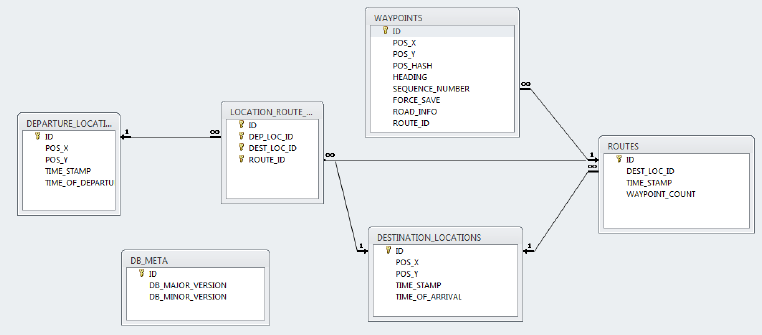
\includegraphics[width=0.9\textwidth]{Figures/baza_date.png}}
  \caption{Structura tabelelor de date și relațiile dintre ele}
\end{figure}

Tabelele din figura de mai sus sunt folosite pentru realiza structura întregii baze de date.
\vspace{6pt}
\\Tabela meta este folosită la identificarea versiunii bazei de date. Acest lucru este necesar pentru a detecta compatibilitatea și pentru a permite migrarea către o versiune mai recentă. 
\vspace{6pt}
\\Datele înregistrate sunt separate în puncte de plecare, destinații, rute și waypoint-uri. O rută este întotdeauna formată din mai multe waypoint-uri, unul sau mai multe puncte de plecare și una sau mai multe destinații. Ruta (waypoint-urile) sunt stocate numai o singură dată, în timp ce toate punctele de plecare și destinațiile sunt stocate. În acest fel, numărul de destinații poate influența probabilitatea rutei.
\vspace{6pt}
\\Accesul la date se face prin SQLite. Toate datele stocate pot fi atât citite cât și modificate.



%% Chapter 3
\stepcounter{cap}


%\arabic(cap)
%-\hspace{8cm}
\mychapter{3}{\arabic{cap}. Arhitectura software}
%\chapter{\arabic{cap}.Software} % Main chapter title

\noindent\rule{14.7cm}{0.4pt}\\
\-\hspace{1cm}Platforma de dezvoltare Unity 3D\\
\-\hspace{1cm}Crearea unei animații în Unity3D\\
\-\hspace{1cm}Limbajul de programare specific plăcii de dezvoltare Arduino\\
\-\hspace{1cm}Platforma Matlab\\
\noindent\rule{14.7cm}{0.4pt}

\label{Chapter3} % For referencing the chapter elsewhere, use \ref{Chapter1} 

%\lhead{\emph\bfseries \textcolor{black!100}{Universitatea \textit{Transilvania} din Braşov \\Facultatea de Inginerie Electrică şi Ştiinţa Calculatoarelor}}
%
%\rhead{\emph\bfseries \textcolor{black!100}{Departamentul Automatică \\și Tehnologia Informației }}

\fancyhead[L]{\fontsize{12}{12}\selectfont\emph\bfseries\textcolor{black!70}{Universitatea \textit{Transilvania} din Braşov \\Facultatea de Inginerie Electrică şi Ştiinţa Calculatoarelor}}

\fancyhead[R]{\fontsize{12}{12}\selectfont\emph\bfseries\textcolor{black!70}{Automatică şi \\ Informatică Aplicată}}

\section{Platforma de dezvoltare Unity 3D}\label{sec3_1}
\-\hspace{1cm}La începutul anilor 2000, trei tineri programatori, fără  mulți bani, au început să codeze și să implementeze cea ce avea să devină una din cele mai populare platforme software din industria jocurilor. Acești trei programatori sunt David Helgson, Joachim Ante și Nicholas Francis, iar proiectul lor a fost inspirat din platforma Apple Final Cut Pro. Final Cut Pro oferea realizatorilor amatori de filme instrumente profesionale la un preț redus, pe aceleași coordonate s-a bazat și Unity, vizând dezvoltatorii amatori de jocuri video.\\
\-\hspace{1cm}O versiune primitivă de Unity a fost lansată în 2005, versiune ce era compatibilă și pe sistemul Windows, nu doar sistemul de operare Mac pentru care s-a dezvoltat inițial. Din 2008 bazându-se pe un real succes, platforma a devenit mult mai complexă, iar vânzările softului le-a permis să angajeze și o duzină de programatori.\\
\-\hspace{1cm}O altă lovitură dată de în 2009 a fost folosirea platformei Unity3D de către Cartoon Network pentru crearea FusionFall, un MMORPG (Massively Multiplayer Online Role Playing Game) pentru copii ce a fost jucat de 8 milioane de persoane. Electronic Arts a folosit în Unity3D în 2009 pentru crearea Tiger Woods PGA Tour Online, chiar Microsoft și Ubisoft au devenit clienți pentru Unity.\\
\-\hspace{1cm}Astăzi Unity are peste 300 de angajați în toată lumea și dezvoltă software pentru iOS, Android, Windows, Mac, Linux, Web browsers, PS3, Xbox 360.  Unity plănuiește suport și pentru Sony’s PlayStation Vita, oferind în acest moment suport pentru Windwos Phone și BlackBerry. Peste 1.8 milioane de programatori folosesc Unity, plug-in-ul pentru browser a fost insatlat de peste 200 de milioane de ori. Dead Trigger și Dead Trigger 2, unele din cele mai complexe grafici pentru jocuri au fost dezvoltate pe baza a Unity3D.\\
Chiar dacă mari nume din industria graficii folosesc Unity, micii dezvoltatori sunt principala mândrie ai dezvoltatorilor acestei platforme, fapt ce se observă din deviza spusă de David Helgson, CEO și co-fondatorul Unity: \textit{”Dorința noastră este să oferim aceleași instrumente și micilor developeri precum granzilor”} \cite{unity}
\begin{figure}[h!]
  \centering
    \centering{%
      \includegraphics[width=0.9\textwidth]{Figures/unity}}
  \caption{Animație Unity}
\end{figure}

\subsection{Editorul Unity}

\-\hspace{1cm}Editorul Unity are împărțită fereastra principală mai multe secțiuni vizibile  imaginea \ref{fig:unity}, ce descrie secțiunile importante.
\begin{figure}[h!]
  \centering
    \centering{%
      \includegraphics[width=0.65\textwidth]{Figures/Editor-tool}}
  \caption{Editorul Unity}\label{fig:unity}
\end{figure}

\-\hspace{1cm}Editorul Unity oferă un mediu \textit{drag and drop}. Pentru dezvoltarea unui joc nu e nevoie obligatoriu de scrierea uni cod într-un limbaj de programare, dar majoritatea proiectelor necesită deprinderi de programare. Unity oferă o diversitate de limbaje de codare precum C\# , JavaScript, sau Boo, pentru dezvoltatorii ce folosesc sintaxa Python. Mediul de dezvoltare este rulat în Mono, o versiune gratis de .NET Framework. Platforma Unity în sine este scrisă în C++,pentru că, din spusele lui Helgson "Animația trebuie să ruleze rapid precum un program C++, dar controlul animației trebuie făcut printr-un limbaj accesibil, oferit de platforma .NET" \cite{unity}.

\subsection{Crearea unei animații în Unity3D}
\-\hspace{1cm}Un joc în Unity este împărțit în mai multe obiecte ale jocului, obiecte ce sunt principalele entități ale animației și au proprietăți speciale, acesta putând fi un personaj, mediu înconjurător sau un efect special. Astfel anumite obiecte dintr-un joc sunt foarte diferite,fiind necesară o repartizare a acestora în containere ce înmagazinează obiecte de același tip.\\
\textbf{Folosirea obiectelor}\\
\-\hspace{1cm}Un obiect dintr-un joc are automat o poziție, rotație și scalare, componente definite de unelta \textit{Transform}, ce determină locația obiectului în spațiul real (3D).\\
\-\hspace{1cm}Prin unelta \textit{Rigidbody}, îi putem adăuga obiectului creat anumite caracteristici ce influențează comportaea inerțială din lumea reală,  parametrii precum  masa sau gravitația, aceștia influnțând comportarea animației spre o comportare realistă.
\begin{figure}[h!]
  \centering
    \centering{%
      \includegraphics[width=0.65\textwidth]{Figures/EmptyGO}}
  \caption{Uneltele \textit{Transform} și \textit{Rigidbody} }
\end{figure}

\subsection{Controlul unei animații în Unity}
\-\hspace{1cm}Chiar și cele mai ușoare jocuri au nevoie de o secțiune de cod într-un limbaj de programare ce va răspunde la intrările venite de la utilizator și organizează evenimentele jocului într-o succesiune dorită de dezvoltator. Secțiunea de cod poate fi folosită pentru a crea efecte grafice sau chiar implementarea unui algoritm de inteligență artificială pentru personajele jocului.\\
\-\hspace{1cm}Codul scris într-un limbaj compatibil .Net creează conexiunea dintre obiectele și acțiunile jocului, implementând  o clasă principală de tip \textit{MonoBehaviour}, ce va fi atșată unui obiect din joc. \\
\-\hspace{1cm}În cadrul clasei $MonoBehavouir$  există două funcții principale. Funcția $Update$, în care se programează acțiunea obiectului în fiecare frame. În cadrul acestei funcții se programează acțiunile de răspuns la intrările introduse de utilizator. Practic, această funcție programează atitudinea obiectului, căreia este asociată, pe tot parcursul jocului. A doua funcție importantă în orice joc,  este funcția $Start$ ce este apelată înainte ca jocul să înceapă, realizând toate inițializările stărilor obiectului, parametrii inițiali cu care va rula jocul în cadrul primei rulării a funcției Update, practic a fiecărui frame al jocului \cite{unity}. 
\begin{lstlisting}
using UnityEngine;
using System.Collections; 

public class MainPlayer : MonoBehaviour {

    // Use this for initialization
    void Start () { 
    
    }
    
    // Update is called once per frame
    void Update () {
    
    }
}
\end{lstlisting}
\-\hspace{1cm}Atașarea comportării setate de codul scris este asignată foarte ușor în cadrul editorului Unity, prin tragerea link-ului scriptului scrs asupra link-ului obiectului din panoul $Hierarchy$. Astfel în cadrul panoului $Inspector$ se poate observa că obectului i-a fost atașat un script, precum în imaginea următoare:
\begin{figure}[h!]
  \centering
    \centering{%
      \includegraphics[width=0.45\textwidth]{Figures/ScriptInInspector}}
  \caption{Confirmarea atașării scriptului }
\end{figure}

\section{Limbajul de programare specific plăcii de dezvoltare Arduino}
\-\hspace{1cm}Pentru a programa microcontroller-ul trebuie să conectată placa Arduino la un computer pe care trebuie instalat mediul de dezvoltare şi driverele necesare. Mediul de dezvoltare este disponibil în mod gratuit pe site-ul producătorului pentru diverse sisteme de operare \cite{arduino}.\\
\-\hspace{1cm}Pentru a configura mediul de dezvoltare arduino pentru sistemul de operare Windows se urmează pașii:
\begin{itemize}
		 \setlength\itemsep{0em}
		 \item se descarcă aplicaţia de pe pagina producătorului şi se dezarhivează într-un director convenabil;
		 \item se conectează placa Arduino la computer printr-un cablu USB asstfel cel puţin un LED ar trebui să se aprindă pe placă;
		 \item se indică locaţia driverului, în general directorul C:/arduino-1.0/drivers;
		 \item se pornește mediul de dezvoltare executând C:/arduino-1.0/arduino.exe;
		 \item se indică modelul plăcii în meniul Tools > Board;
		 \item se indică portul pe care s-a conectat placa Arduino în meniul Tools > Serial Port;
		 \item se elaborează scriptul ce se dorește a fi încărcat pe microcontroller;
		 \item se încarcă programul pe placă: File > Upload.
 		\end{itemize}

\subsection{Structura limbajului arduino}
\-\hspace{1cm}Limbajul folosit este o variantă simplificată de C/C++, ameliorată cu diverse biblioteci specifice platformei Arduino. Este foarte uşor de folosit pentru oricine are experienţă de programare în orice limbaj cât de cât structurat. De altfel, puteţi constata cât de simplu este analizând exemplul următor, care aprinde și stinge la anumite inervale un led:
\begin{lstlisting}
 1. /*
 2.   Blink
 3.   Turns on an LED on for one second, then off for one second, repeatedly.
 5.   This example code is in the public domain.
 6.  */
 7. 
 8. void setup() {                
 9.   // initialize the digital pin as an output.
10.   // Pin 13 has an LED connected on most Arduino boards:
11.   pinMode(13, OUTPUT);     
12. }
13. 
14. void loop() {
15.   digitalWrite(13, HIGH);   // set the LED on
16.   delay(1000);              // wait for a second
17.   digitalWrite(13, LOW);    // set the LED off
18.   delay(1000);              // wait for a second
19. }
\end{lstlisting}

\-\hspace{1cm}Au fost definite două funcţii, $setup()$ (liniile 8-12) şi $loop()$ (liniile 14-19). Aceste două funcţii trebuie să fie prezente în orice program.\\
Funcţia $setup()$ este executată o singură dată, la iniţializarea plăcii (de fiecare dată când este alimentată, de fiecare dată când încărcaţi un program nou şi de fiecare dată când resetaţi placa).În programul nostru, funcţia setup() face un singur lucru: declară pinul 13 (adică pinul digital 13) ca pin de ieşire. Dacă vă amintiţi de mai sus, pinul 13 este conectat şi la LED-ul de pe placă.\\
\-\hspace{1cm}Funcţia $loop()$ se execută apoi la infinit, fără pauză. Dacă se doresc pauze sau încetiniri ale programului se pot scrie în acestă secțiune. În exemplul de mai sus funcţia $loop()$ realizează următoarele:
\begin{itemize}
		 \setlength\itemsep{0em}
		 \item linia 15: scrie "1" la pinul 13 (adică din acest moment pinul respectiv va fi alimentat cu 5V);
		 \item linia 16: aşteaptă 1000 de milisecunde, adică o secundă; nu uitaţi, pinul 13 este alimentat, deci LED-ul de pe placă este aprins;
		 \item linia 17: scrie "0" la pinul 13 (adică din acest moment pinul respectiv nu va mai fi alimentat);
		 \item linia 18: aşteaptă din nou o secundă (dar de data asta pinul 13 nu mai este alimentat, deci LED-ul este stins).
 		\end{itemize}
 		
\subsection{Vizulaizarea datelor în ediorul arduino}
\-\hspace{1cm}Arduino permite vizualizarea datelor procesate de mocrocontroller prin intermediul unui modul serial, care se sincronizează prin intermediul codului, unde se setează o viteză de transfer a datelor prin comunicație serială. Astfel utiliztorul poate avea acces la datele procesate de arduino pe calculatorul propriu, modalitate foarte eficientă de evaluare a comportării procesului.
\begin{figure}[h!]
  \centering
    \centering{%
      \includegraphics[width=0.8\textwidth]{Figures/serial_modul}}
  \caption{Datele procesate de arduino și afișate prin modulul serial }
\end{figure}
\\ \\ \\
\section{Platforma Matlab}\label{sec3_3}
\-\hspace{1cm}MATLAB® (MATtrix LABoratory) este un pachet de programe de înaltă performanţă,
interactiv, destinat calculului matematic, ştiinţific şi ingineresc. MATLAB integrează
calcul, programare şi vizualizare, într-un mediu de lucru prietenos, soluţionarea problemelor
presupunând folosirea notaţiilor matematice clasice. Utilizarea programului MATLAB
include: \\
\-\hspace{1cm}• Matematică şi calcul numeric\\
\-\hspace{1cm}• Programare şi dezvoltare de algoritmi\\
\-\hspace{1cm}• Modelare şi simulare\\
\-\hspace{1cm}• Analiză de date, exploatarea rezultatelor şi vizualizare\\
\-\hspace{1cm}• Grafică ştiinţifică şi inginerească\\
\-\hspace{1cm}• Dezvoltare de aplicaţii software, incluzând construcţie de interfeţe grafice cu utilizatorul
(GUI)\\
\-\hspace{1cm}MATLAB este un produs al companiei americane The Mathworks, Inc.
[http://www.mathworks.com] şi lucrează sub Windows, Unix, LINUX şi Machintosh.
MATLAB include toate facilităţile unui limbaj complet de programare, admiţând interfeţe
cu limbajul de programare C, C++ şi FORTRAN.

\-\hspace{1cm}MATLAB a cunoscut o puternică evoluţie în decursul ultimilor ani, reprezentând astăzi
în mediile universitare o unealtă standard de calcul, fiind asociată diverselor cursuri
introductive sau avansate în matematică, ştiinţă şi inginerie. În industrie, MATLAB este
recunoscut ca un mijloc de investigaţie numerică performant, utilizat în sprijinul unei
activităţi de cercetare, dezvoltare şi analiză de înalt nivel. \\
\-\hspace{1cm}Versiunea completă a pachetului de programe MATLAB conţine o întreagă familie de
module specifice, denumite tool-box-uri, respectiv blockset-uri, care permit rezolvarea unor
aplicaţii din diverse domenii cum ar fi: maşini, aparate şi acţionări electrice, control de
sistem, aplicaţii DSP, procesarea materialelor şi electro-tehnologii, procesare de semnal,
mecanică, industria aeronautică şi de automobile, statistică, finanţe şi multe altele. \\
\-\hspace{1cm}Aceste module sunt colecţii de funcţii MATLAB (M-files), uşor de asimilat, care extind
puterea de calcul a pachetului de programe MATLAB în vederea rezolvării unor clase
particulare de probleme. Colecţia de module MATLAB conţine: Simulink, DSP, Control
System, SimPowerSystems, SimMechanics, Data Acquisition, Fuzzy Logic, Image
Processing, Partial Differential Equations, Neural Network, Optimization, System
Identification, Financial, Statistics, Communications, Database, Virtual Reality  \cite{matlab}. 

\subsection{Structura sistemului MATLAB }
\textbf{Mediul de dezvoltare}

\-\hspace{1cm}Acesta este alcătuit dintr-un set de unelte care facilitează
folosirea funcţiilor şi fişierelor MATLAB. Multe dintre acestea reprezintă de fapt interfeţele grafice şi includ fereastra principală MATLAB sau MATLAB Desktop, fereastra de comenzi sau Command Window, fereastra ce memorează istoria comenzilor sau Command History, şi browser-ele de Help, Workspace, Files, Search Path.

\textbf{Biblioteca de funcţii matematice MATLAB}

\-\hspace{1cm} Aceasta constă într-o vastă colecţie de algoritmi de calcul, pornind de la funcţii elementare precum sumă, sinus, cosinus şi
aritmetică complexă, pană la funcţii mai sofisticate precum inversare de matrici, calcul de
valori proprii, funcţii Bessel, şi transformata Fourier.

\textbf{Limbajul MATLAB} 

\-\hspace{1cm}Limbajul MATLAB este un limbaj matrice/vector de înalt nivel
ce include instrucţiuni de control al buclelor, funcţii, structuri de date, comenzi de
intrare/ieşire şi instrucţiuni de programare orientată pe obiecte. Limbajul MATLAB permite
atât ”programarea superficială” pentru crearea rapidă a unor mici programe de calcul
specifice, cât şi "programarea în detaliu" în vederea dezvoltării unor programe complexe de
nivel superior.

\textbf{Handle Graphics®}.

\-\hspace{1cm}Handle Graphics reprezintă sistemul de grafică MATLAB şi
include atât comenzi de înalt nivel pentru vizualizarea 2D şi 3D a datelor, procesare de
imagini, animaţie şi grafică, cât şi comenzi de jos nivel ce permit personalizarea completă a
reprezentărilor grafice şi construirea integrală a interfeţelor grafice (GUI) pentru aplicaţiile
MATLAB.

\textbf{MATLAB Application Program Interface (API)}.

\-\hspace{1cm}Aceasta este o bibliotecă ce permite
scrierea programelor C şi Fortran ce interacţionează cu MATLAB. Biblioteca conţine
facilitaţi de apel de subrutine din MATLAB (dynamic linking), de apelare a MATLAB-ul ca
pe o maşină de calcul, şi de citire şi scriere de fişiere MAT-files \cite{matlab}. 

\begin{figure}[h!]
  \centering
    \centering{%
      \includegraphics[width=0.8\textwidth]{Figures/matlab1}}
  \caption{Editorul Matlab}
\end{figure}

\section{Conexiunea dintre Arduino și calculator}
\-\hspace{1cm}Placa de dezvoltare Arduino prezintă facilități gândite pentru utilizatorii care se simt mult mai confortabil programând într-un limbaj de nivel înalt  (Java, C\#, Phyton, Ruby, PHP) . Aceaste facilități sunt  realizate de comunicația serială , dintre plăcile Arduino și calculatoarele clasice, prin intermediul căreia datele captate de la senzori și/sau datele procesate de microcontroller-ul plăcii arduino vor fi transferate calculatorului unde, cu ajutorul unor limbaje de programare de nivel înalt, se pot realiza aplicații mult mai complexe, atât la nivel hardware cât și software. Tot aceași facilitate poate fi adusă prin realizarea unei comunicații de tip ethernet, dar această facilitate ridică costurile structurii hardware, și este dependentă de conexiunea la internet.
\begin{figure}[h!]
  \centering
    \centering{%
      \includegraphics[width=0.8\textwidth]{Figures/arduinoToPc}}
  \caption{Conexiunea dintre placa Arduino și calculator}
\end{figure}

\-\hspace{1cm}Datele sunt transmise în flux continuu, într-un format de tip string separat printr-un caracter, în general virgulă.La nivelul limbajului de programare folosit pe calculator trebuie făcută citirea datelor și interpretarea acestora în funcție de semnificația acestora \cite{arduino}.

\subsection{Conexiunea dintre placa de dezvolatre Arduino și Unity}\label{sec3_4_1}
\-\hspace{1cm}Comunicarea dintre Arduino și Unity este realizată cu ajutorul librăriei CmdMessenger, ce face legătura între Arduino și limbajele .Net, implicit și editorul specific platformei Unity, Mono, editor ce e compatibil cu implementările C\# \cite{unity}.\\
Această librărie facilitează:\\
\-\hspace{1cm}1. Trimiterea și primirea comenzilor în ambele sensuri.\\
\-\hspace{1cm}2. Adăugarea de argumente comenzilor.\\
\-\hspace{1cm}3. Generarea de funcții de reacție ca răspuns la anumite comenzi primite.\\
\-\hspace{1cm}4. Transferul datelor bidirectional.\\

Formatul codului de citire a datelor prin intermediul portului serial, în cadrul editorului Mono, arată astfel:

\begin{lstlisting}
using System;
using System.IO.Ports;

class MainClass
{	
	public static void Main(string[] args)
	{
		SerialPort sport = new SerialPort("/dev/ttyUSB0", 9600);

		if (sport != null)
		{
			if (sport.IsOpen)
				{
					sport.Close();
				}
		}

		Console.WriteLine("Arduino Serial Test");

		sport.Open();

		while(true)
		{		
			Console.WriteLine(sport.ReadLine());
		}
	}
}
\end{lstlisting}

\subsection{Conexiunea dintre placa de dezvolatre Arduino și Matlab}\label{sec3_4_2}
\-\hspace{1cm}Pentru a facilita transferul dintre Arduino și platforma Matlab se folosește pachetul MATLAB Support Package.Acest pachet se bazează pe un program ce rulează pe placa Arduino, ce ascultă comenzi venite prin intermediul portului serial, execută comenzile și, la nevoie, returnează un răspuns.\\
În imaginea următoare se poate vedea o parte din comenzile folosite în cadrul comunicației seriale \cite{matlab}.

\begin{figure}[h!]
  \centering
    \centering{%
      \includegraphics[width=0.7\textwidth]{Figures/MatlabToArduino}}
  \caption{Conexiunea dintre placa Arduino și calculator}
\end{figure}
%% Chapter 1
\stepcounter{cap}
%\chapter{cap1}
\label{cap4}

\mychapter{4}{Capitolul \arabic{cap} \\ STRUCTURA BAZEI DE DATE}
%\chapter{\arabic{cap}.Introducere} % Main chapter title

\label{Chapter4} % For referencing the chapter elsewhere, use \ref{Chapter1} 

\thispagestyle{fancy}

%-----------------------------------------------------------------
\section{Tabelele de date}


\begin{figure}[h!]
  \centering
    \centering{%
      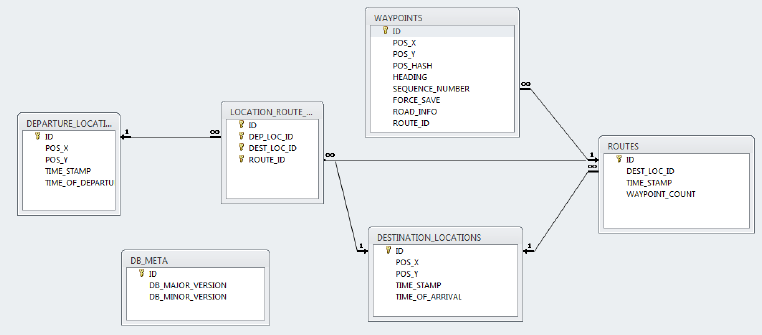
\includegraphics[width=0.9\textwidth]{Figures/baza_date.png}}
  \caption{Structura tabelelor de date și relațiile dintre ele}
\end{figure}

Tabelele din figura de mai sus sunt folosite pentru realiza structura întregii baze de date.
\vspace{6pt}
\\Tabela meta este folosită la identificarea versiunii bazei de date. Acest lucru este necesar pentru a detecta compatibilitatea și pentru a permite migrarea către o versiune mai recentă. 
\vspace{6pt}
\\Datele înregistrate sunt separate în puncte de plecare, destinații, rute și waypoint-uri. O rută este întotdeauna formată din mai multe waypoint-uri, unul sau mai multe puncte de plecare și una sau mai multe destinații. Ruta (waypoint-urile) sunt stocate numai o singură dată, în timp ce toate punctele de plecare și destinațiile sunt stocate. În acest fel, numărul de destinații poate influența probabilitatea rutei.
\vspace{6pt}
\\Accesul la date se face prin SQLite. Toate datele stocate pot fi atât citite cât și modificate.


 
% Chapter 1
\stepcounter{cap}
%\chapter{cap1}
\label{cap5}

\mychapter{5}{Capitolul \arabic{cap} \\ DESCRIEREA ALGORITMILOR}
%\chapter{\arabic{cap}.Introducere} % Main chapter title

\label{Chapter5} % For referencing the chapter elsewhere, use \ref{Chapter1} 

\thispagestyle{fancy}

%-----------------------------------------------------------------

\section{Învățarea rutelor} 
Rutele sunt învățate printr-un mecanism inteligent. Acest lucru are avantajul de a reduce semnificativ baza de date și de a accelera încărcarea datelor.

	\subsection{Reducerea waypoint-urilor} 
	Criteriile pentru excluderea waypoint-urilor sunt:
	\begin{enumerate}
	 \setlength\itemsep{0em}
		\item Vehiculul nu și-a schimbat orientarea semnificativ (valoare standard: > 15$^{\circ}$)
		\item Pozițiile sunt apropiate una de cealaltă (valoare standard: > 200m)
	\end{enumerate}
	
	Valorile standard pot fi configurate  înaintea procesului de compilare.
	
	
	\subsection{Verificarea rutelor duble} 
	În cazul în care ruta curentă are o secțiune similară cu o rută deja invățată, unitatea software PNavDataManager va detecta secțiune respectivă și va stoca numai waypoint-urile situate după aceasta. În schimb, toate destinațiile sunt memorate. Criteriile pentru a detecta o astfel de rută sunt:
	
		\begin{enumerate}
	 \setlength\itemsep{0em}
		\item Destinația noii rute trebuie să fie situată într-o rază de 1km față de locația vechii destinații
		\item Punctul de start al noii rute trebuie să fie situată într-o rază de 1km față de punctul de plecare vechii destinații
		\item Toate waypoint-urile noii rute trebuie:
				\begin{enumerate}
				 \setlength\itemsep{0em}
					\item Să fie situat într-o anumită rază față de punctul de start al vechii rute
					\item Sau să fie situat într-o anumită rază față de destinația vechii rute
					\item Sau să fie situat într-o anumită rază față de un waypoint al vechii rute
				\end{enumerate}
	\end{enumerate}

Pragurile pot fi configurate înaintea procesului de compilare.


	\subsection{Filtrarea rutelor inutile}
	În timpul învățării, rutele prea scurte (< 2km) nu vor fi stocate deoarece acest lucru ar însemna faptul că utilizatorul este destul de aproape de destinație.
	\vspace{6pt}
  \\Totodata, rutele foarte lungi (> 200km) vor fi de asemenea exclude din stocare deoarece ele nu reprezintă rute uzuale.
	\vspace{6pt}
  \\Pragurile pot fi configurate înaintea procesului de compilare.
	
\section{Eliberarea de spațiu} 
Dacă pragul setat inițial pentru dimensiunea maximă a bazei de date este atins, se va activa funcția de eliberare a spațiului. Aceasta va șterge obiectele cele mai vechi pentru a crea loc pentru obiectele noi.

\section{Furnizarea predicțiilor} 
Pentru ca predicțiile să fie disponibile sunt necesari doi pași.
\vspace{6pt}
\\Primul pas reprezintă încărcarea datelor revelante, în timp de al doilea constă în prioritizarea lor.

	\subsection{Filtrarea datelor}
	Pentru o încărcare selectivă și mai rapidă a datelor din unitatea PNavDataStorage, sunt create interogări. Sunt definiți trei pași în filtrare, unde pasul următor se excută doar în cazul în care cel curent nu a returnat destule rezultate:
		\begin{enumerate}
				 \setlength\itemsep{0em}
					\item Filtrarea rutei în funcție de distanța de la poziția curentă la waypoint-urile rutelor
					\item Filtrarea rutei în funcție de distanța de la poziția curentă la punctele de start ale rutelor
					\item Filtrarea rutelor în funcție de timpul scurs până la ajungerea la destinație
		\end{enumerate}

	Toate rutele ce duc la o destinație situată la o distanță mai mică de 1km față de poziția actuală sunt ignorate deoarece utilizatorul aproape a ajuns la eventuala destinație.
	\vspace{6pt}
	\\În cazul predicțiilor baza pe timp, modulul furnizează o predicție fără a cunoaște ruta, ci doar destinația sa. Un astfel de caz ar fi cel în care utilizatorul a condus pe o rută în intervalul luni-miercuri, însă in ziua de joi a pornit de la o altă locație. Astfel, bazat pe timp, modulul prezice destinația fără a ști ruta corespunzătoare acesteia.
	
	
		\subsection{Frecvența predicției de rute}
		De obicei, waypoint-urile furnizate de modul de predicție sunt transformate într-o rută ce folosește drumuri din hartă, fapt ce durează câteva secunde.
		Pentru a nu supraîncărca sistemul de navigație cu prea multe predicții, dezolvatorul poate seta timpul minim dintre două predicții. Acestă setare se poate efectua chiar în timpul rulării.
		
		\subsection{Numărul maxim de predicții}
		Pentru a putea suporta multiple platforme, modulul permite setarea numărului maxim de rute prezise ce apar deoadată. Acestă setare se poate efectua chiar în timpul rulării.
		
		\subsection{Prioritizarea predicțiilor}
		Există mai multe criterii pentru a stabili prioritatea unei rute. 
		
		\begin{table}[!h]
		\caption{Criterii de prioritizare pentru predicția bazată pe rute}
		\centering
		\begin{tabular}{ | m{2,7cm} | m{3,6cm} | m{3,22cm} | m{3,22cm} | m{1,4cm} | }
		\hline
		\textbf{Criteriu} & \textbf{Descriere} & \textbf{Min (0\% probabilitate)} & \textbf{Max (100\% probabilitate)} & \textbf{Pondere} \\ 
		\hline
		 Frecvența rutei & Numărul de utilizări al unei rute & Niciodată & Folosită de mai mult de 10 ori & 4 \\
		\hline
		 Frecvența rutei într-un anumit interval de timp & Numărul de utilizări al unei rute într-un anumit interval de timp (de la -1 oră la +2 ore) față de ora curentă & Niciodată & Folosită de mai mult de 10 ori & 1 \\
		\hline
		 Frecvența rutei într-o anumită zi & Numărul de utilizări al unei rute în ziua curentă din săptămână & Niciodată & Folosită de mai mult de 10 ori & 1 \\
		\hline
		 Frecvența rutei într-un anumit grup de zile & Numărul de utilizări al unei rute într-un anumit grup de zile (e.g. luni-vineri)& Niciodată &  Folosită de mai mult de 10 ori  & 1 \\
		\hline
		 Ultima utilizare a unei rute & Diferența dintre ultima utilizare a rutei și ora/data curentă & >4 săptămâni & <2zile & 3 \\
		\hline
		 Distanța până la destinație & Distanța dintre poziția actuală și destinație & >100km & 0km & 1 \\
		\hline
		\end{tabular}
		\label{table:tabel_predictii}
		\end{table}
		
		
		\subsection{Predicții bazate pe filtrarea rutei în funcție de distanța de la poziția curentă la waypoint-urile rutelor}
		Criteriile definite în tabela ~\ref{table:tabel_predictii}, ``Criterii de prioritizare pentru predicția bazată pe rute'' sunt extinse prin adăugarea următoarelor criterii:
		
		\begin{table}[!h]
		\caption{Criterii de prioritizare pentru predicția bazată pe rutele din jurul unei poziții}
		\centering
		\begin{tabular}{ | m{2,7cm} | m{3,6cm} | m{3,22cm} | m{3,22cm} | m{1,4cm} | }
		\hline
		\textbf{Criteriu} & \textbf{Descriere} & \textbf{Min (0\% probabilitate)} & \textbf{Max (100\% probabilitate)} & \textbf{Pondere} \\ 
		\hline
		 Distanța până la rută & Distanța dintre poziția actuală și waypoint-urile rutei &> 1km & 0km & 1 \\
		\hline
		 Direcția către rută & Diferența dintre orientarea waypoint-urilor și direcția de navigare & 180$^{\circ}$ & 0$^{\circ}$ & 1 \\
		\hline
		\end{tabular}
		\end{table}
		
		
		\subsection{Predicții bazate pe filtrarea rutei în funcție de distanța de la poziția curentă la punctele de start ale rutelor}
		Criteriile definite în tabela ~\ref{table:tabel_predictii}, ``Criterii de prioritizare pentru predicția bazată pe rute'' sunt extinse prin adăugarea următoarelor criterii:
		
		\begin{table}[!h]
		\caption{Criterii de prioritizare pentru predicția bazată pe filtrarea rutele în funcție de distanța până la punctul de start al rutei}
		\centering
		\begin{tabular}{ | m{2,7cm} | m{3,6cm} | m{3,22cm} | m{3,22cm} | m{1,4cm} | }
		\hline
		\textbf{Criteriu} & \textbf{Descriere} & \textbf{Min (0\% probabilitate)} & \textbf{Max (100\% probabilitate)} & \textbf{Pondere} \\ 
		\hline
		 Distanța până la punctul de start al rutei & Distanța până la cel mai apropiat punct de start al rutei &> 3km & 0km & 1 \\
		\hline
		\end{tabular}
		\end{table}
		
		\subsection{Predicții bazate pe filtrarea rutei în funcție de timpul scurs până la ajungerea la destinație}
		Pentru acest caz sunt folosite criteriile definite în tabela ~\ref{table:tabel_predictii}, ``Criterii de prioritizare pentru predicția bazată pe rute''.
		
		
		
		


	 
% Chapter 1
\stepcounter{cap}
%\chapter{cap1}
\label{cap6}

\mychapter{6}{Capitolul \arabic{cap} \\ MANAGEMENTUL ERORILOR}
%\chapter{\arabic{cap}.Introducere} % Main chapter title

\label{Chapter6} % For referencing the chapter elsewhere, use \ref{Chapter1} 

\thispagestyle{fancy}

%-----------------------------------------------------------------

\section{Tipuri de erori} 
\begin{itemize}
 \setlength\itemsep{0em}
	\item Erori de secveță
	\item Erori apărute la accesarea bazei de date
	\item Bază de date coruptă
\end{itemize}


\section{Detectarea erorilor}
Erorile sunt raportate pentru fiecare apel către și dinspre interfata modului de predicție. Toate funcțiile returnează un număr ce corespunde unui tip de eroare.

	\subsection{Erori de secvență}
	O mașină de stare va verifica încălcarea ordinii secvețelor.
	
	\subsection{Erori la accesarea bazei de date}
	Trebuie evaluate rezultatele funcțiilor native de accesare ale bazei de date.

	\subsection{Bază de date coruptă}
	Trebuie evaluate rezultatele funcțiilor native de accesare ale bazei de date.
	
	
\section{Tratarea erorilor}
În funcție de tipul de eroare, aceasta poate fi prevenită pe viitor sau nu de către dezvoltator.
\vspace{6pt}
\\Există erori de secvență precum ``Înainte de apelarea funcției X este necesară pornirea unității software PNavPredictor''. Se poate întâmpla de asemenea ca atunci când dezvoltatorul pornește procesul de predicție de două ori consecutiv sa fie întampinat de eroarea ``Procesul de predicție se află deja în curs de rulare''.
În astfel de cazuri este clar cum se pot preveni erorile.
\vspace{6pt}
\\Mai sunt însă și cazuri ce nu pot fi tratate de către dezvoltator. Astfel de erori sunt cele precum ``Baza de date este coruptă'', ce pot să apară în cazul în care fișierul de sistem folosit pentru stocarea datelor este corupt. În aceste situații datele stocate anterior nu mai pot fi recuperate, toate informațiile referitoare la rute fiind definitiv piedute.



 
%\stepcounter{cap}

\mychapter{7}{\arabic{cap}. Rezultate experimentale}

%\chapter{\arabic{cap}.Determinarea orientării pe baza filtrului AHRS} % Main chapter title

\label{Chapter7} % For referencing the chapter elsewhere, use \ref{Chapter1}
\noindent\rule{14.7cm}{0.4pt}\\
\-\hspace{1cm} Analiza datelor citite de senzorii inerțiali\\
\-\hspace{1cm} Rezultatele algoritmilor de determinare a orientării\\
\-\hspace{1cm} Rezultatele determinării orientării pe baza unghiurilor lui Euler și a filtrului \\
\-\hspace{1cm}AHRS\\
\noindent\rule{14.7cm}{0.4pt}

%\lhead{\emph\bfseries \textcolor{black!100}{Universitatea \textit{Transilvania} din Braşov }}
%
%\rhead{\emph\bfseries \textcolor{black!100}{Departamentul Automatică \\și Tehnologia Informației }}

\fancyhead[L]{\fontsize{12}{12}\selectfont\emph\bfseries\textcolor{black!70}{Universitatea \textit{Transilvania} din Braşov \\Facultatea de Inginerie Electrică şi Ştiinţa Calculatoarelor}}

\fancyhead[R]{\fontsize{12}{12}\selectfont\emph\bfseries\textcolor{black!70}{Automatică şi \\ Informatică Aplicată}}

%----------------------------------------------------------------------------------------
\-\hspace{1cm}Principiile de determinare a orientării în spațiul tri-dimensional,  enunțate în capitolele anterioare pot fi dovedite prin fuziunea dintre datele captate de structura hardware și procesarea acestora pe baza structurii software cu scopul determinării parametrilor orientativi ce descriu un corp în spațiul terestru.

\-\hspace{1cm}Pe baza arhitecturi hardware expusă în capitolul 2 ce are ca scop captarea parametilor inerțiali ce pot fi procesați prin mai multe platforme software, platforme ce pot fi rulate la nivelul plăcii de dezvoltare sau la nivelul calculatorului. În funcție de comlexitatea algoritmului și facilitățile dorite folosit se aleg platformele optime și dispozitivele pe care acestea rulează.

\-\hspace{1cm}Independent de algoritmii de determinare implementați și platforma hardware pe care rulează aceștia, este nevoie de o reprezentre a detelor de intrare, eventual a datelor preliminare, și a rezultatelor procesării pentru a observa comportările sistemului și a face analize asupra acestora. În acest scop,  în cadrul acestui proiect sa folosit platforma Matlab expusă în subcapitlolul \ref{sec3_3}, ce citește datele de la nivelul structurii hardware, pe baza comunicației seriale detaliate în subcapitolul \ref{sec3_4_2} și realizează o reprezentare grafică a acestora.

\-\hspace{1cm}Pentru simularea orientării determinate de algoritmii de filtrarea și modelare a parametriilor inerțiali sa folosit platforma Unity3D detaliată în subcapitolul \ref{sec3_1} ce primește datele procesate de algoritmii rulați pe placa de dezvoltare Arduino prin conexiunea expusă în secțiunea  \ref{sec3_4_1}.

\section{Analiza datelor citite de senzorii inerțiali}
\-\hspace{1cm}Asupra datelor citite de senzorii inerțiali sau formulat o serie de formulări matematice a comportării acestora având în vedere toți factorii perturbatori ai mediului înconjurător.

\subsection{Analiza parametrilor în regim static}
\-\hspace{1cm}În cadrul acestei secțiuni se observă comportărole intrărilor sistemului în cazul în care senzorul nu este deviat din poziția inițială. Astfel rezultă următoarele caracteristici ale datelor giroscopului:
\begin{figure}[h!]
  \centering
    \centering{%
      \includegraphics[width=0.7\textwidth]{Figures/GyroData}}
  \caption{Parametrii giroscopului în regim staționar}
\end{figure}

\-\hspace{1cm}În această reprezenatre a datelor furnizate de giroscop se observă că viteza unghiulară are valoarea zero pe toate cele trei direcții spațiale, giroscopul ne fiind scos din starea inițială.

\-\hspace{1cm}Aceste caracteristici nu mai sunt valabile pentru valorile accelerometului care generează o repartiție a semnalului vizibilă în figura \ref{fig:gyro}. În această figură se observă că se adeveresc principile enunțate în capitolul \ref{Chapter1}, cu privire cărora accelerația este afectată de zgomote. Principala influență asupra parametriilor accelerației e adusă de influența forței gravitaționale exerciate de Pământ. Precum sa enunțat pe   parcursul lucrării se observă că cea mai importantă influență a gravitației este asupra datelor generate de acceleormetru pe axa $z$, paralelă cu gravitația. Pe acestă direcție senzorul detectează a accelerație constantă, dar diferită cu mult de zero, valoarea reală a acesteia.
\-\hspace{1cm}Prin această comportare se poate observa că, perturbația instalată de gravitație asupra axei paralele pe direcția acesteia, trebuie compensată în scopul obținerii unei comportări reale.
\begin{figure}[h!]
  \centering
    \centering{%
      \includegraphics[width=0.7\textwidth]{Figures/AccData}}
  \caption{Parametrii accelerometrului în regim staționar}\label{fig:gyro}
\end{figure}
\subsection{Analiza datelor de intre în regim dinamic}
\-\hspace{1cm}În această secțiune se încearcă observarea distribuței parametrilor accelerometrului și giroscopului în funcție de orientarea senzorului. Această evaluare este o evaluare pur subiectivă, pe baza repartiției semnalelor se poate observa o orientare posibilă, dar nu sigură sau măsurabilă.

\-\hspace{1cm}Astfel în imaginea următoare se poate observa pe baza semnalelor provenite de la giroscop un model al rotaților realizat de senzor.
\begin{figure}[h!]
  \centering
    \centering{%
      \includegraphics[width=0.6\textwidth]{Figures/GyroDinam}}
  \caption{Datele furnizate de giroscop în regim dinamic}
\end{figure}

\-\hspace{1cm}Pe baza imaginii anterioare se poate observa, în diferite secțiuni, o rotație accentuată. Astfel în prima secțiune se observă valori ridicate ale vitezei unghiulare realizate pe axa $x$, putând presupune că senzorul realizează o rotație în jurul axei $x$. În a doua secțiune a imaginii se poate observa o fluctuație a valorilor semnalului pe axa $y$, putănd presupune ca sunt rezultate ale rotație în jurul axei $z$. Ultima secțiune a imaginii conține fluctuații importante ale semnalului furnizat de axa $z$ a giroscopului, comporate ce poate determina o rotație în jurul axei $z$. 

\-\hspace{1cm}Pe baza presupunerilor anterioare se poate  presupune o orientare, operând anumite valori de threshold se poate spune că între anumite valori avem ununghi $\alpha$ în raport cu axa $x$, dar acesta este o evaluare nesigură și orientativă.

\-\hspace{1cm}Semnalele echivalente accelerometrului, din  modelul mișcărilor dezbătut anterior, sunt reprezentate în imaginea:
\begin{figure}[h!]
  \centering
    \centering{%
      \includegraphics[width=0.9\textwidth]{Figures/AccDinam}}
  \caption{Datele furnizate de accelerometru în regim dinamic}
\end{figure}

\-\hspace{1cm}Din repartiția semnalelor realizată anterior nu se poate determina un model al accelerației, dar se observă fluctuații importante ale valorilor accelerației pe axa $z$, valori afectate de accelerația gravitațională. În funcție de rotațiile realizate de corp se poate observa că la un moment dat și celealte axe ale sistemului sunt paralele cu vectorul accelerației gravitațiomnale, putându-se presupune existența unor perturbații ridicate ce afectează accelerațiile de pe axele $x$ respectiv $z$.

\section{Rezultatele algoritmilor de determinare a orientării}
\-\hspace{1cm}Presupunerile anterioare asupra unei posibile orientări a corpului în spațiul 3D pe baza fluctuaților parametrilor giroscopului reprezinta ipoteze nesigure și imprecise. În scopul formulării unei unei expresii precise și sigure a orientării unui corp sau elaborat o serie de algoritmi matematici ce determină, pe baza parametriilor inerțiali, o formulare veridică a orientării în spațiul tri-dimensional.

\-\hspace{1cm}O parte din algoritmii matematici, elaborați în decursul timpului, ce pot determina orientarea 3D sau amintit în secțiunea \ref{cap1_3}. Dar principile implementate în acest proiect au fost bazate pe metoda matricei cosinusului (DCM) și unghiurile lui Euler, respectiv metoda filtrului AHRS pe baza cuaternionilor.

\subsection{Rezultatele determinării orientării pe baza unghiurilor lui Euler și a filtrului AHRS}
\-\hspace{1cm}Reprezentarea sub forma unghiurilor lui Euler a fost detaliată în subcapitolul \ref{cap4_1}, enunțând rotațiile realizate în funcție de cele trei axe , în care se reprezintă rotația în sensul acelor de ceasornic  funcție de axa $z$ (yaw), rotația în funcție de axa $y$ (pitch),rotația în fucție de axa $x$ (roll).

\-\hspace{1cm}Determinarea orientării pe baza unghuirilor lui Euler generează rezultate bune fară un volum mare de calcul, dar principala problemă a acestei reprezentări este generată de defetul principal al acestei metode, acesta este principiul blocării gimbal este reprezentat de cazul în care două inele axiale se plasează pe același plan, moment în care sistemul 3D se transforma într-un model 2D.

\-\hspace{1cm}În scopul evitării acestui defect al metodei unghiurilor lui Euler s-a încercat implementarea unui filtru AHRS, un filtru dezvoltat din metoda filtrului Kalman și filtrul Kalman extins detaliate în capitolul 6, ce se bazează pe descrierea spațiului tri-dimensional printr-un vector al cuaternionilor dezbătut în secțiunea \ref{cap4_2}. Această reprezentare a spațiului 3D sub forma de cuaternioni elimină blocarea gimbal, îmbunătațind calitatea determinării orientării.

\-\hspace{1cm}Filtrul AHRS dezvoltat în capitolul 7 generează o calculare a orientării, implicând și componenta câmpului magnetic al pământului, copmensând foarte bine erorile de măsurare ale giroscopului și reușind să elimine proceseze componenta accelerației gravitaționale în scopul îmbunătățirii performanțelor.
  
\-\hspace{1cm}Comparând metoda filtrului AHRS cu metoda filtrării Kalman se observă ca versiunea filtrului AHRS realizată de Madgwick are o viteză de procesare mai bună decât filtrul Kalman, realizănd calcule matematice mult mai reduse, generând rezultate asemănătoare calitativ. 

\subsubsection{Rezultatele determinării orientării în regim static}
\-\hspace{1cm}Rezultatele experimentale pot fi analizate prin reprezentarea rezultatelor generate de cele două metode în același grafic, astfel putându-se observa diferențele acestora.

\-\hspace{1cm}Imaginile următoare reprezintă detectarea orientării în regim static, paketul de senzori ne fiind scos din echilibru:
\begin{figure}[h!]
  \centering
    \centering{%
      \includegraphics[width=0.7\textwidth]{Figures/Roll}}
  \caption{Reprezentarea unghiului în raport cu axa $x$}
\end{figure}

\begin{figure}[h!]
  \centering
    \centering{%
      \includegraphics[width=0.7\textwidth]{Figures/Pitch}}
  \caption{Reprezentarea unghiului în raport cu axa $y$}
\end{figure}

\-\hspace{1cm}În imaginile precedente se poate observa că, dupa calibrare,  cele două metode au o comportatrea asemănătoare, observăndu-se că senzorul are o poziție apropiată de zero grade în raport cu axa $x$, și $y$.
 
\-\hspace{1cm}Această comportare va fi diferită în momentul în care se încercă detectare unghiului în raport cu axa $z$, această reprezentare se poate analiza în imaginea:
\begin{figure}[h!]
  \centering
    \centering{%
      \includegraphics[width=0.9\textwidth]{Figures/Yaw}}
  \caption{Reprezentarea unghiului în raport cu axa $z$}
\end{figure}

\-\hspace{1cm}Din reprezentarea orintării pachetului de senzori față de axa $z$ a sistemului spațial se observă că în cazul metodei unghiurilor lui Euler stabilizarea se face mult mai rapid decât timpul de stabilizare al metodei AHRS, dar această are un rezultat mult mai bun decât cel al al metodei unghiurilor lui Euler. În cazul acesta unghiul cu raportat față de axa $z$ este apropiat de $90^0$, observându-se că filtrul AHRS se stabilizează la această valoare.  

\subsubsection{Rezultatele determinării orientării în regim dinamic}
\-\hspace{1cm}Determinarea orientării în regim dinamic este mult mai dificilă datorită schimbărilor bruște ale parametrilor senzorilor. Comportarea orientării aplicând cele două metode, duce la detectarea unei orientări similare în raport cu axa $x$ și $y$, observându-se că orientarea detectată cu metoda unghiurilor lui Euler generează un răspuns mult mai liniar, fără a detecta fluctuațile rapide. 

\-\hspace{1cm}Analizând orientările detectate de filtrul AHRS se poate observa că acesta detectează fluctiații mult mai dese ale miscărilor unghiulare realizate de sistem. Acest poate fi folositor pentru precizie, dar poate fi deranjant pentru stabilitate și constanță.

\-\hspace{1cm}Analiza realizată anterior se bazează pe următoarele figuri ce descriu comparativ comportarea sistemului aplicând cele două metode: 
\begin{figure}[h!]
  \centering
    \centering{%
      \includegraphics[width=0.7\textwidth]{Figures/RollDim}}
  \caption{Reprezentarea orientării în raport cu axa $x$}
\end{figure}

\begin{figure}[h!]
  \centering
    \centering{%
      \includegraphics[width=0.7\textwidth]{Figures/PitchDim}}
  \caption{Reprezentarea orientării în raport cu axa $y$}
\end{figure}

\-\hspace{1cm}Precum în cadrul comportării în regim stabil, reprezentarea  orientării dinamice în raport cu axa $z$ a sistemului 3D prezintă soluții diferite genertate de cele două metode. Pe baza comportării semnalului se poate observa că metoda filtrului AHRS are o comportare foarte diferită în raport cu metoda ungiurilor lui Euler, în special în primele perioade de timp, când filtrul AHRS se calibrează și se stabilizează. După stabilizarea modelului AHRS cele două modele genereaza un model asemănător al semnalului, dar rezultatul filtrului AHRS est mai precis comparativ cu cel al modelului unghiurilor lui Euler.

\begin{figure}[h!]
  \centering
    \centering{%
      \includegraphics[width=0.9\textwidth]{Figures/YawDim}}
  \caption{Reprezentarea orientării în raport cu axa $z$}
\end{figure}

\-\hspace{1cm}Pentru a vizualiza orientarea mai apropiat de realitatea mișcărilor sa realizat o animație în limbajul Matlab care preia datele orientării si le transpune într-o animație ce arată orientarea tridimensională. Un cadru al acestei animații este în imaginea:
 \begin{figure}[h!]
  \centering
    \centering{%
      \includegraphics[width=0.9\textwidth]{Figures/AHRS_anim}}
  \caption{Reprezentarea orientării în 3D}
\end{figure} 
%\stepcounter{cap}

\mychapter{8}{\arabic{cap}. Concluzii și dezvoltări ulterioare}

%\chapter{\arabic{cap}.Determinarea orientării pe baza filtrului AHRS} % Main chapter title

\label{Chapter8} % For referencing the chapter elsewhere, use \ref{Chapter1}
\noindent\rule{14.7cm}{0.4pt}\\
\-\hspace{1cm} Concluziile proiectului\\
\-\hspace{1cm} Direcții de dezvoltare ulterioară\\
\noindent\rule{14.7cm}{0.4pt}

%\lhead{\emph\bfseries \textcolor{black!100}{Universitatea \textit{Transilvania} din Braşov }}
%
%\rhead{\emph\bfseries \textcolor{black!100}{Departamentul Automatică \\și Tehnologia Informației }}

\fancyhead[L]{\fontsize{12}{12}\selectfont\emph\bfseries\textcolor{black!70}{Universitatea \textit{Transilvania} din Braşov \\Facultatea de Inginerie Electrică şi Ştiinţa Calculatoarelor}}

\fancyhead[R]{\fontsize{12}{12}\selectfont\emph\bfseries\textcolor{black!70}{Automatică şi \\ Informatică Aplicată}}

%----------------------------------------------------------------------------------------
\section{Concluziile proiectului}
\-\hspace{1cm}Acest proiect a constituit o introducere în domeniul determinării orientării în spațiul tri-dimensional și a raportării corpurilor, aflate în mișcare, la condițile impuse de forțele terestre. Astfel accelerația gravitațională și componenta câmpului magnetic reprezentând un factor important în cadrul orientării corpurilor.

\-\hspace{1cm}Demersurile făcute în cadrul acestui proiect au dus la identificarea unui model de structură hardware ce poate capta parametrii de accelerometru, giroscop și magnetometru. Această structură este disponibilă tuturor doritorilor, la prețuri reduse. Placa de dezvoltare Arduino reprezintă o structură hardware robustă, complexă , rapidă și foarte fiabilă, fiind bine documentată de producător, astfel este foarte ușor de învățat structura hardware și facilitățile acesteia. Analizând facilitățile pachetului de senzori inerțiali AltIMU-10, se poate spune că este un pachet de senzori foarte complex, cu performanțe foarte bune, având componente ce pot măsura date la o fregvență ridicată, facilitate ce este foarte folosiroare în aplicațiile în timp real.  

\-\hspace{1cm}Elaborând concluzii asupra structurii software, s-a observat că există foarte multe limbaje de programare ce pot fi folosite în combinație cu placa de dezvoltare Arduino, facilitățile comunicației seriale fiind foarte folositoare, astfel putem spune că programarea software se poate realiza întru-un limbaj de nivel înalt, transferul codului și interpretarea lui în limbaj C/C++ putând fi făcută cu ajutorul unor librării specifice. Această facilitate aduce structurii hardware o flexibilitate importantă, iar structurii software o aplicabilitate complexă.

\-\hspace{1cm}Cea mai provocatoare parte a acestui proiect a fost reprezentată de determinarea algoritmilor pentru determinarea orientării. Această secțiune a dus la studii amănunțite a algoritmilor folosiți și dezvoltați în domeniile aplicabile orientării. Astfel primul algoritm studiat a fost algoritmul unghiurilor lui Euler, principiu ce face baza orientării în spațiul 3D și care are performanțe bune vizibiele prin experimentele folosite, fiind implementabil în aplicațiile în timp real, datorită timpului de răspuns foarte rapid și timpului scurt de stanbilizare.
Studierea mai amănunțită a acestui principiu a scos la iveală o problemă importantă a acestui algoritm, reprezentată de pringimiul blocării gimbal. Blocarea gimbal face ca sistemul să se blocheze în momentul în care orientarea sistemului și face ca două planuri ale axelor de coordonate să fie paralele, atunci sistemul devenind unul 2D, fiind nevoie de o miscare necontrolată pentru deblocare. Principiul blocării gimbal face ca modelul ungiurilor lui Euler să fie un model problematic în determinarea orientării 3D.

\-\hspace{1cm}Pentru a evita problemele evidențiate de principiul unghiurilor lui Euler s-a observat că, în multe studii sa folosit reprezentarea spațiului 3D în forma cuaternionilor, o extindere matematică a numerelor complexe, iar orientarea pe baza acestora se face printr-o filtrare Kalman a datelor inerțiale, astfel se reduc influențele gravitației și câmpului magnetic terestru, orientaea fiind determinată mult mai precis prin elaborarea unei estimării a acestei analizănd starea precedentă, rezultând un control mult mai bun. Această metodă pare ideală, dar problema ei este reprezentată de complexitatea calculelor și multitudinea de iterații, fapt ce o duce la întârzieri, ce afectează implementarea într-o aplicație în timp real.

\-\hspace{1cm}Aprofundând studiile sa observat că aceste întârzieri ale filtrului Kalman pot fi evitate printr-un filtru derivat din filtrul Kalman, filtrul AHRS elaborat de Mahony și îmbunătățit de Madgvick, care implementează mai puține calcule și iterații, astfel rezultă un răspuns mai bun al sistemului, la performanțe asemanătoare filtrului Kalman.
   
\-\hspace{1cm}Prin implementarea metodelor unghiurilor lui Euler și algoritmului AHRS s-a observat că cele două metode prezintă rezultate asemănătoare în determinarea orientării în funcție de axele $x$ și $y$, diferența principală este observată la determinarea orientării axei $z$, în care metoda filtrului AHRS are rezultate mult mai precise, dar cu un timp de stabilizare a semnalului mult mai mare decât cel al metodei Euler.
 
\-\hspace{1cm}Pe baza acestor concluzii experimentale se poate spune că metoda unghiurilor lui Euler este cea mai bună pentru determinarea orientării 2D, dar în cazul în care se dorește monitorizarea orientării în funcție de axa $z$ este nevoie de un filtru ce compensează componenta accelerației gravitaționale, a influenție câmpului magnetic și a erorilor giroscopului, cel mai eficient algoritm fiind expus în filtrul AHRS.

\section{Direcții de dezvoltare ulterioară}
\-\hspace{1cm}Pe baza realizărilor acestui proiect, și obsrvării altor aplicții ale metodelor studiate în această aplicație, dar și prin prisma dezvoltării sistemelor de acest tip se pot trasa mai multe direcții de dezvoltare.

\-\hspace{1cm}O direcție de dezvoltare ar duce la compnesarea unui neajuns al aplicației curente. Acest neajus este legat de conectarea cablată între calculator și arhitectura hardware. Rezolvarea acestei probleme poate fi făcută prin integrarea unei componente ce furnizează conexiunea la internet, în cadrul plăcii de dezvoltare Arduino. Astfel printr-o conexiune TCP/IP se poate realiza conexiune datelor la nivel de LAN. Tot această direcție de dezvoltarre poate fi făcută prin dezvoltarea aplicație pe o platforma Rasberry Pi, care conține implicit un modul ce permite conexiunea wireless, iar sistemul de operare Linux, folosit de această placă de dezvoltare este mult mai stabil, si permite mai multe facilități legate de tipul conexiunii, menționând și timpul de calcul mult mai eficient. 

\-\hspace{1cm}O altă direcție de dezvoltare este reprezentată de îmbunătățirile ce pot fi aduse, cu scopul implementării în cadrul aplicațiilor Unity3D, astfel se poate dezvolta pe baza algoritmilor dezvoltați în acest proiect, și prin îmbunătățirea structurii hardware, un prototip de mănușă ce va oferii utilizatorului o experiență, în animația 3D, conformă cu mișcările realizate de mâna și degetele sale. Astfel jocul dezvoltat va fi mult mai interactiv, calite ce poate fi sporită prin adăugarea unei componente haptice, în cadrul acestei mănuși. Această componetă oferindu-i utilizatorului un răspuns tactil la acțiunile realizate de el în cadrul jocului.

\-\hspace{1cm}Precum s-a observat în secțiunea de introducere a proiectului, studiile de determinare a orientării se folosesc intens în proiectele aerospațiale. Pe baza studiilor și cunoștințelor dobândite în acest proiect se poate trasa un obiectiv de realizare unui quadocopter ce va fi controlat prin miscările mâinii utilizatorului. Acestă dezvoltare este una foarte complexă avănd în vedere că implică și controlul motoarelor, pe baza orientării, dar reprezintă o provocare extrem de interesantă.



\end{document}  